\section{Design Requirements \& Hardware Implementation} \label{sec:hardware}\label{sec:design_requirements}

\subsection{Purpose}
The CALibration Insertion System (CALIS) deploys radioactive gamma and neutron sources inside the LSV to study and calibrate the \tpc\ and the \lsv\ detector response and neutron detection efficiency. This complements and extends internal the physics reach of the laser calibrations and internal calibration sources. 
%The goal with the CALibration source Insertion System (CALIS) is to study and calibrate the detector response of the \tpc\ and the \lsv\ as well as the detection efficiency of internal neutrons interacting in the \tpc\ and \lsv\ using radioactive gamma and neutron sources. 

The \lsv\ may be accessed through one of four gate valves in CRH, which are approximately 6 m above the center of the LSV. Each gate valve connects to an organ pipe 15 cm in diameter which leads through the WCV and opens into the LSV, 80 cm off the TPC's vertical Z-axis, as shown in Fig.~\ref{fig:CALIS_photos}.

%=6145=70+120+400+3455+20+251+1372+457 from http://darkside-docdb.fnal.gov:8080/cgi-bin/RetrieveFile?docid=858&filename=NoFlyZone-DS50_vers02.pdf&version=14
For \tpc\ calibration the radioactive source has to be positioned in immediate contact with the cryostat, in order to minimize rate losses through absorption. This is especially important for low energy sources such as $^{57}$Co (122 keV). 

\subsection{Deployment \& Articulation Mechanism}\label{sec:DeploymentArticulation}
%focus on the mechanism --- protection provided by the housing is discussed below:
The requirement of physical contact between the source holder and the cryostat precludes a single cable solution deployed from within a glove box as used in several other scintillator experiments \cite{Banks:2014hra, Huang:2013uxa}. %\cite{KamLAND-MiniCal, DayaBay_zaxis}. 
As shown in Figs. \ref{fig:CALIS_photos} and \ref{fig:CALISMechanism} our apparatus consists instead of an enclosure, which has been installed in CRH. The deployment device is attached to this enclosure through two stainless steel cables wound around cable spools. These cables both lower the device into the \lsv and articulate the source arm, allowing the calibration source to be brought into contact with the cryostat.
\begin{figure}[htbp]
 \centering
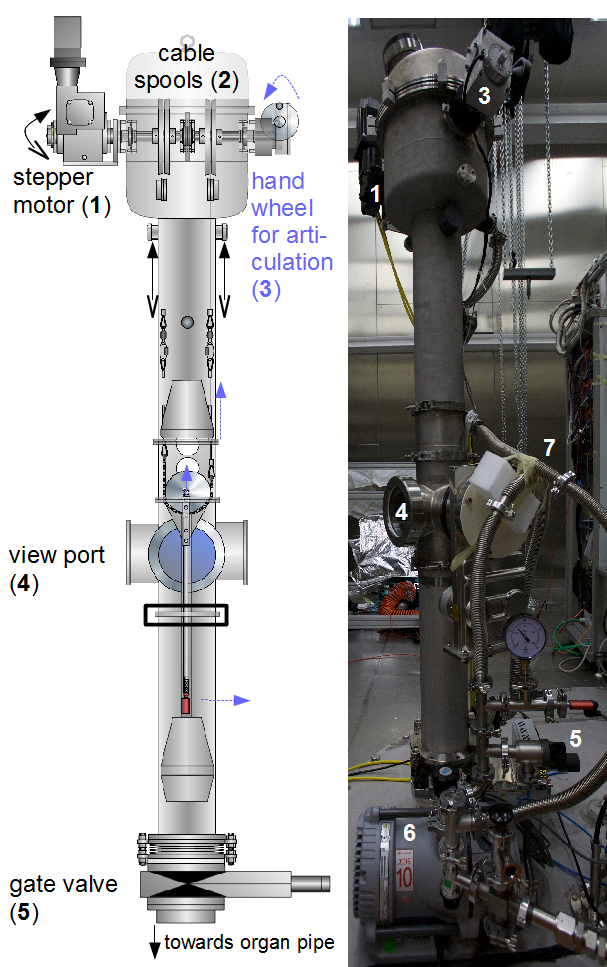
\includegraphics[width=0.7\textwidth]{Figures/CALIS_overview.png}
 %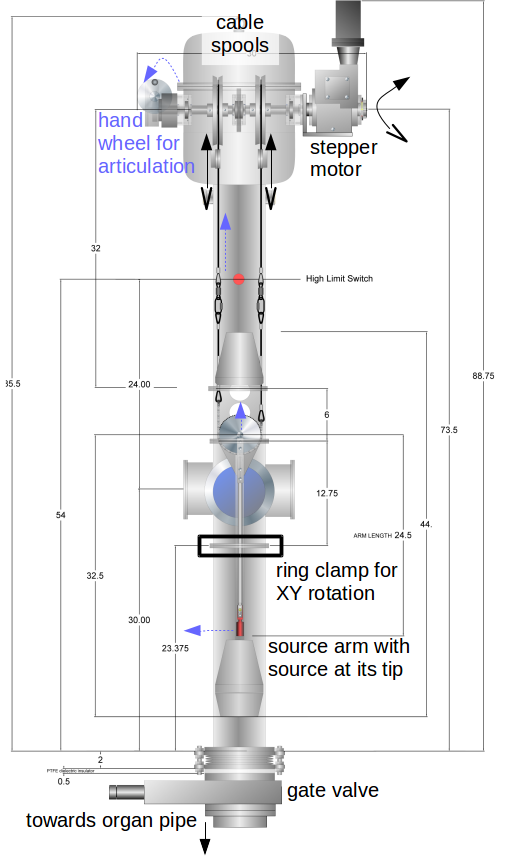
\includegraphics[width=0.68\textwidth]{Figures/CALISDimensions.png}
 %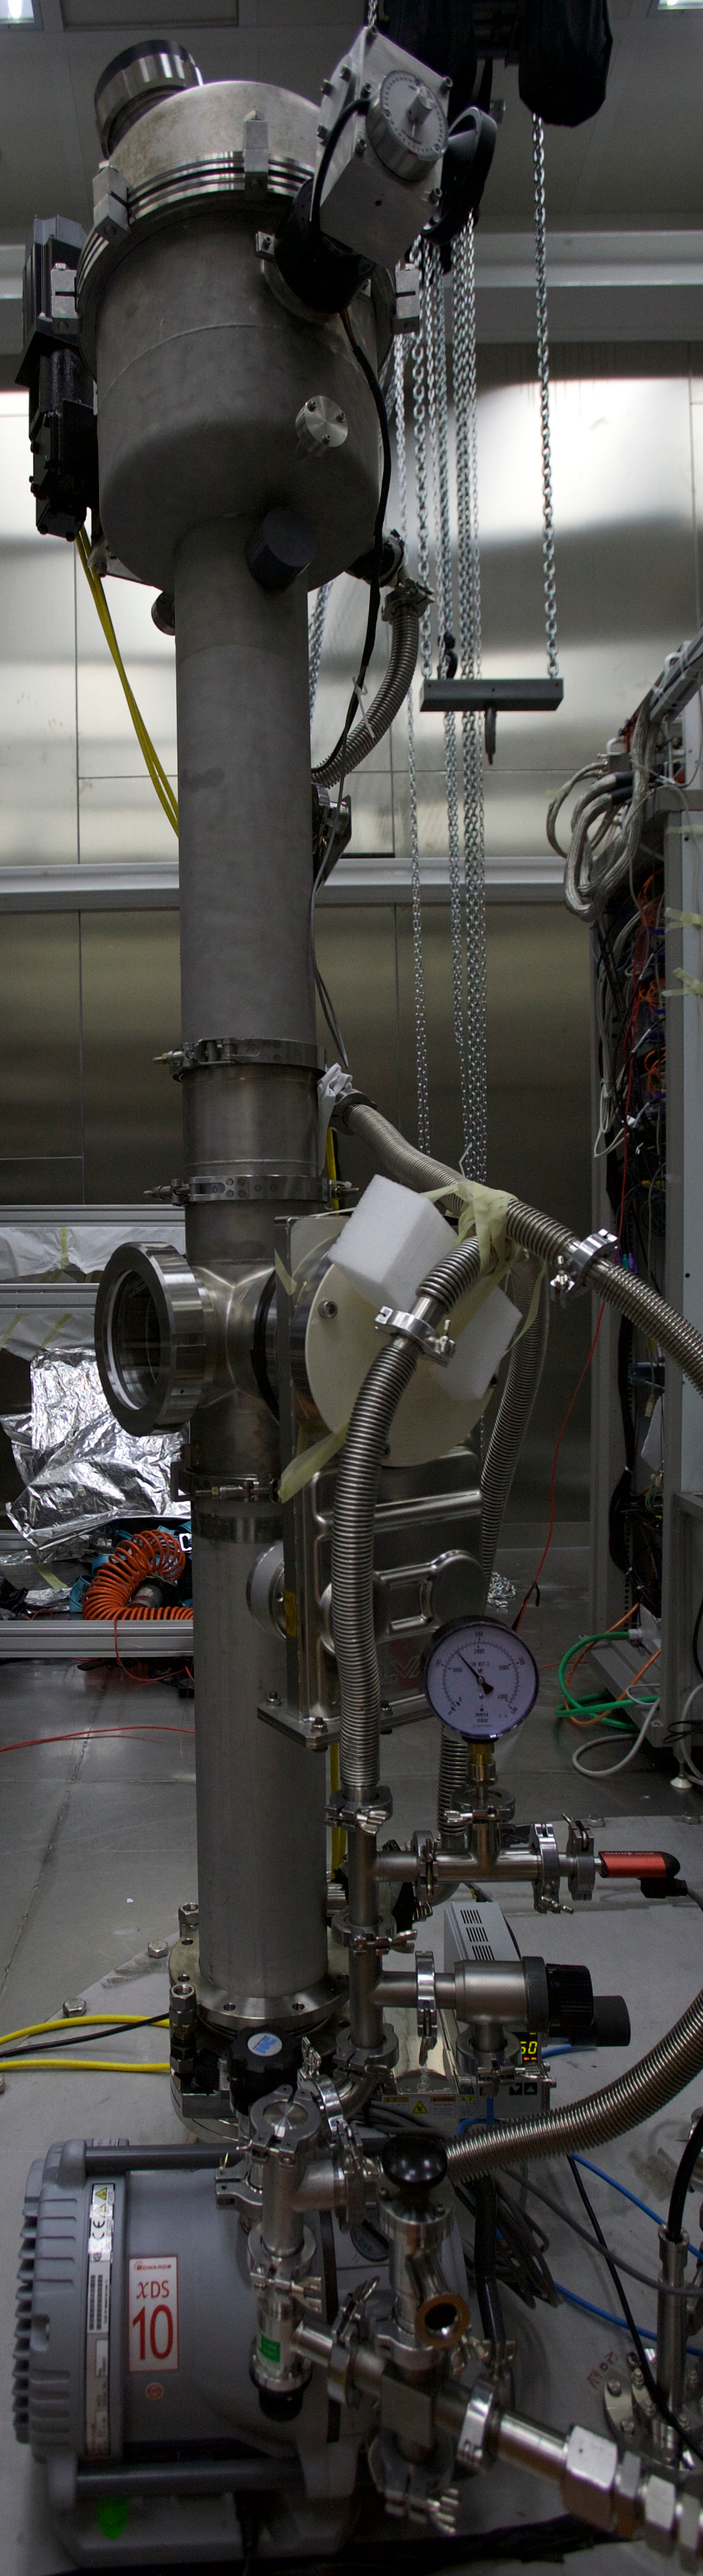
\includegraphics[width=0.30\textwidth]{Figures/CALIS_overview_IMG_3763.jpg}
 \caption{Mechanical drawing of CALIS showing the housing and the deployment device in its home position. The total height is approx.~240 cm including the gate valve.) The two modes of operation are illustrated: In order to move the deployment device down into the LSV or back up the stepper motor moves both cable spools (2) simultaneously. \textcolor{blue}{In order to articulate, the articulation wheel (3) is rotated manually, which affects only the right spool, thereby shortening the right cable with respect to the left cable thereby articulating the arm and lifting the pivot center.} The amount of lifting and the amount of rotations until a horizontal articulation is reached has been calibrated prior to installation in CRH (Sec.~\ref{sec:Testing}). In the photograph the vacuum pump (6) and tubing (7) are shown, which are part of the evacuation and purging system (Sec.~\ref{sec:EvacPurge}). \label{fig:CALISDimensions}\label{fig:CALISMechanism}\label{fig:gearDrawing}\label{fig:flushing_purging}
}
\end{figure}

\begin{figure}[htbp]
 \centering
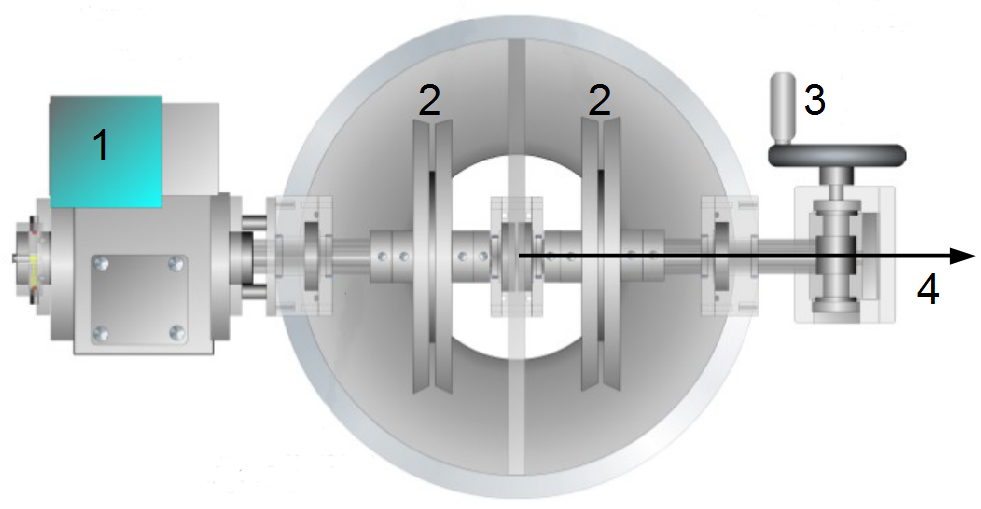
\includegraphics[width=0.9\textwidth]{Figures/gearDrawing_withNumbers}
  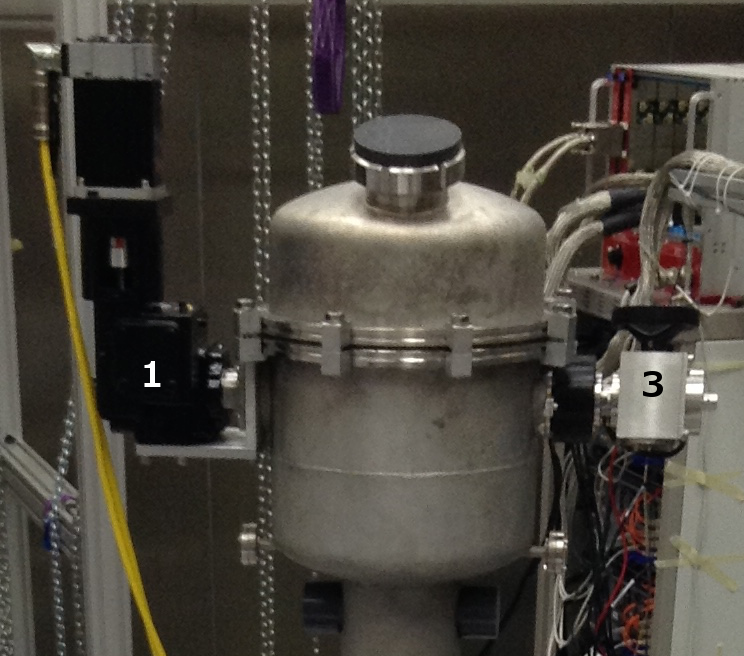
\includegraphics[width=0.46\textwidth]{Figures/CALIS_head.png}
  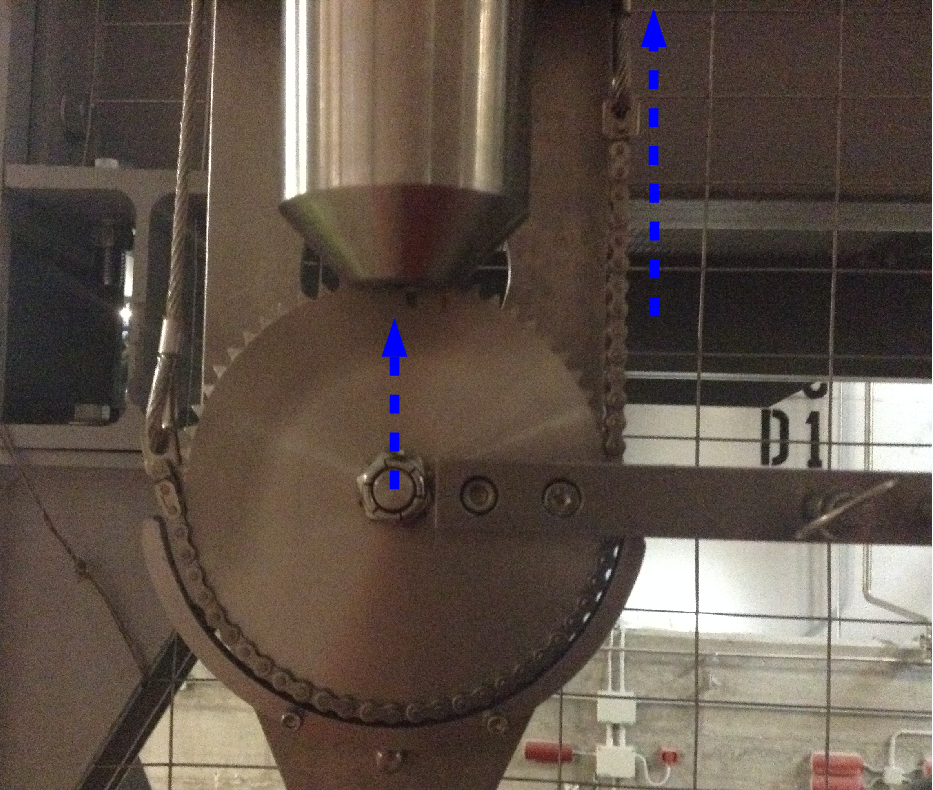
\includegraphics[width=0.48\textwidth]{Figures/gearArticulated.png}
  \caption{\textit{top}: Inside view of the drive mechanism's components seen from the top of CALIS. The stepper motor inside the motor housing (1) drives both cable spools (2) concurrently, thereby lowering the calibration device into the \lsv. An absolute encoder provides the deployment device's current position. The hand wheel (3) turns the right spool only, thereby transfering the rotation of the articulation wheel into a (de)articulation of the source arm (\textit{bottom right}). Arrow (4) in the sketch points in same direction as the horizontally articulated arm. The chain has a guard rail, ensuring the chain can never come off the gear.}
  \label{fig:sourceArmRotation}
\end{figure} 

A stepper motor moves both cable spools concurrently and sends the deployment device into the \lsv. An absolute encoder provides its current position, even in absence of power. The stepper motor is controlled via a simple graphical LabVIEW interface, run on a dedicated laptop, in which the current Z-position is shown and a target Z-position can be provided by the operator. Z-positions are given in motor step counts, an arbitrary unit which has been calibrated outside CRH in meters (Fig.~\ref{fig:z_test}) and relative to the TPC using calibration data's t-drift distributions (Fig.~\ref{fig:SourcePosition}).

\begin{figure}[htbp]
 \centering
 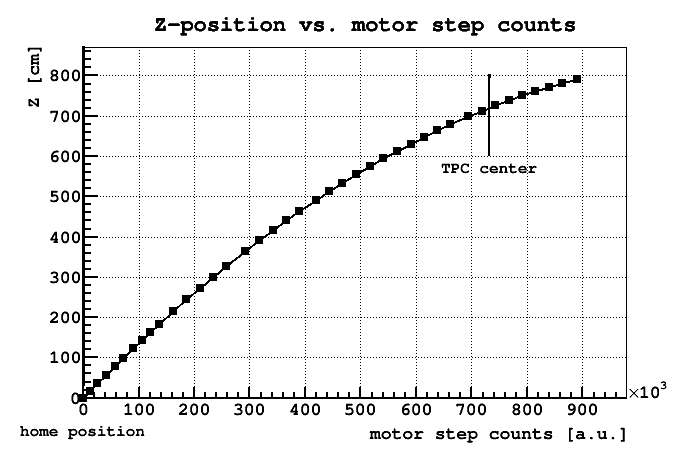
\includegraphics[width=0.59\textwidth]{Figures/MSC_Z}
%at 0.6 textwidth the plot is on a separate page
 \caption{Plot of the deployment device's Z-position versus motor step counts. The non-linear correspondence between number of steps and cable length deployed arises as follows: As the cables wind around their spools, the winding radius changes, increasing as the deployment device is lifted and decreasing as it is lowered. A motor step count corresponds to a fixed angular distance \textit{d$\theta$}, yet the amount of cable deployed during this motor step is \textit{winding radius $\cdot$ d$\theta$}. As the winding radius changes as a function of Z-position, the fraction of deployed cable per motor step count changes. The home position is at 0, the TPC center is reached after more than 7 m of travel into the \lsv, the maximum depth is reached at nearly 8 m.}
 \label{fig:z_test}
\end{figure}

\label{sec:Nonlinearity:MotorStepCounts}
Arm articulation is done manually via the articulation wheel. This affects only the cable spool close to the articulation wheel, the right one in Fig.~\ref{fig:sourceArmRotation}, thereby shortening the right cable with respect to the left cable and engaging the gear through a chain (Fig.~\ref{fig:sourceArmRotation}). As a result the source arm is articulated and the pivot center is lifted. A non-linearity between motor steps and cable length arising from the change in winding radius on cable spools affects also the amount of rotation required by the hand wheel for horizontal source arm articulation.
Degrees on the articulation wheel corresponding to a horizontal articulation have been calibrated as a function of cable length prior to installation in CRH.

Articulation and a movement in Z-direction are mutually exclusive since arm articulation leads to more wound up cable on the spool close to the articulation wheel with respect to the other. If then in Z-movement mode both spools would be rotated simultaneously with the same angular speed, the cable close to the articulation wheel would wind up faster than the other, leading to a build up of difference in cable length and the deployment device would only be hanging on one cable. In order to avoid an imbalanced Z-movement the arm has to be dearticulated fully before a change in Z-position can be initiated. This is enforced by an electric switch preventing Z-movement, which is disengaged only when the source arm is fully dearticulated (i.e.~ hanging vertically). 

%Discussion:
% why no permanent tube?
% To complement studies of nuclear recoils with neutron sources ($^{241}$Am$^{9}$Be and $^{241}$Am$^{13}$C), it is planned to deploy a 

\subsection{CALIS Enclosure \& Scintillator}

Besides providing mechanical support for the deployment device via the cable spools, the CALIS enclosure is an important interface between the radon-free clean room CRH and the \lsv, through which sources are exchanged. 
The enclosure protects the liquid scintillator (LS) and eliminates human contact with any traces of harmful LS vapor (Fig.~\ref{fig:CALISMechanism}). It plays the same role as a glove box for similar calibration systems yet with a narrower foot print inside CRH. The liquid scintillator is a mixture of PC and TMB\footnote{The concentration of TMB has varied during campaigns (see Sec.~\ref{sec:CalibCampaigns}).} with the wavelength shifter PPO \cite{Agnes:2015qyz}. %\cite{vetoPaper}. 
It may not get exposed to oxygen or water as is present in normal clean room air. Contamination of the LS with $^{222}$Rn and its long-lived radioactive daughters has to be avoided, too. 

Going up from the gate valve on which CALIS has been installed, there is a teflon disk that can electrically isolate CALIS from ground, even though during normal operations the CALIS housing is connected to ground. A tripod with a bellow has been used to vertically align the enclosure right after installation on the gate valve. The bellow is connected to a 59.4 cm long cylindrical stainless steel enclosure pipe. It has the same diameter as the organ pipe (15 cm) and is connected to the view port by a ring clamp, which plays a critical role for rotations in the XY-plane (see Sec.~\ref{sec:XYrotation}). The view port can be opened for handling the source arm and exchanging calibration sources. Everything above the ring clamp forms the upper assembly. It features a stainless steel cylindrical enclosure housing the cable drive mechanism, including the cable spools, the stepper motor and the articulation mechanism already described in Sec.~\ref{sec:DeploymentArticulation}. 

\subsubsection*{Vacuum evacuation (flushing) and nitrogen purging system}\label{sec:EvacPurge}
One of this system's most important safety features is making sure that TMB and PC residue on the deployment device are extracted from CALIS and vented prior to opening the access ports to access the source arm. This is  important for safe working conditions inside CRH as well as for the scintillator and its radiopurity. 

After the source arm insertion and view port closure the inside of the CALIS housing is filled with normal air, that is damaging to the scintillator. A sequence of evacuations and nitrogen purges reduces the fraction of normal air including its contaminants in the air-N$_2$ mixture to negligible levels. Only after this sequence is finalized, the gate valve is opened and the deployment device is introduced into the \lsv. Evacuation is achieved with a vacuum pump and the exhaust air is removed through dedicated vent lines (Fig.~\ref{fig:flushing_purging}).

At the end of a calibration campaign, after the deployment device has returned to its home position inside the enclosure and the gate valve has been closed, scintillator vapor, and in particular TMB, has to be removed prior to opening the view port. Again a sequence of n evacuation and nitrogen purges is employed. By lowering the pressure inside of CALIS below the TMB and PC vapor pressure, the scintillator evaporates and gets removed through the vacuum pump vent line. Once pressure inside the housing stays consistently below the vapor pressure of TMB all scintillator has been removed and the view port can be opened to access the source arm.
 
%\begin{figure}[htbp]
%\centering
% 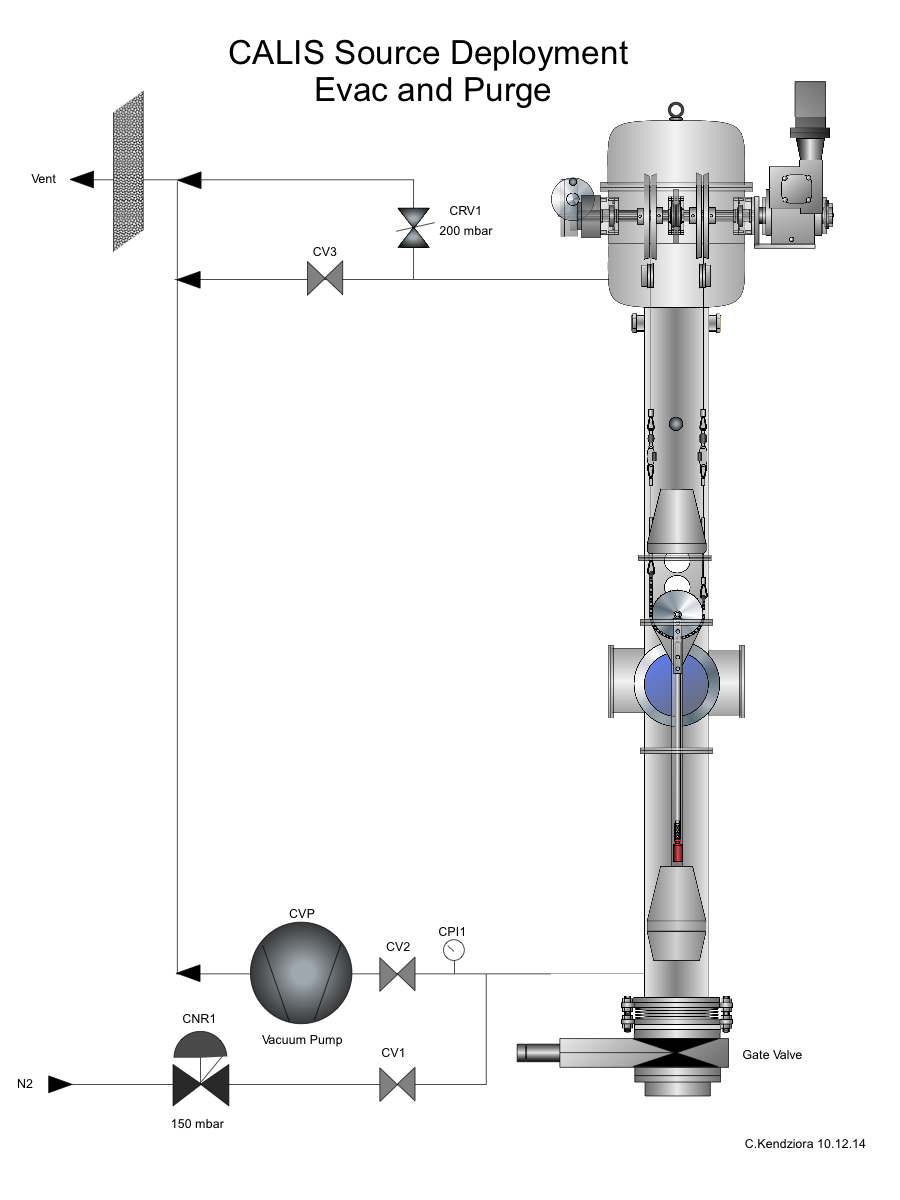
\includegraphics[width=0.73\textwidth]{Figures/GasSystem.png}
% 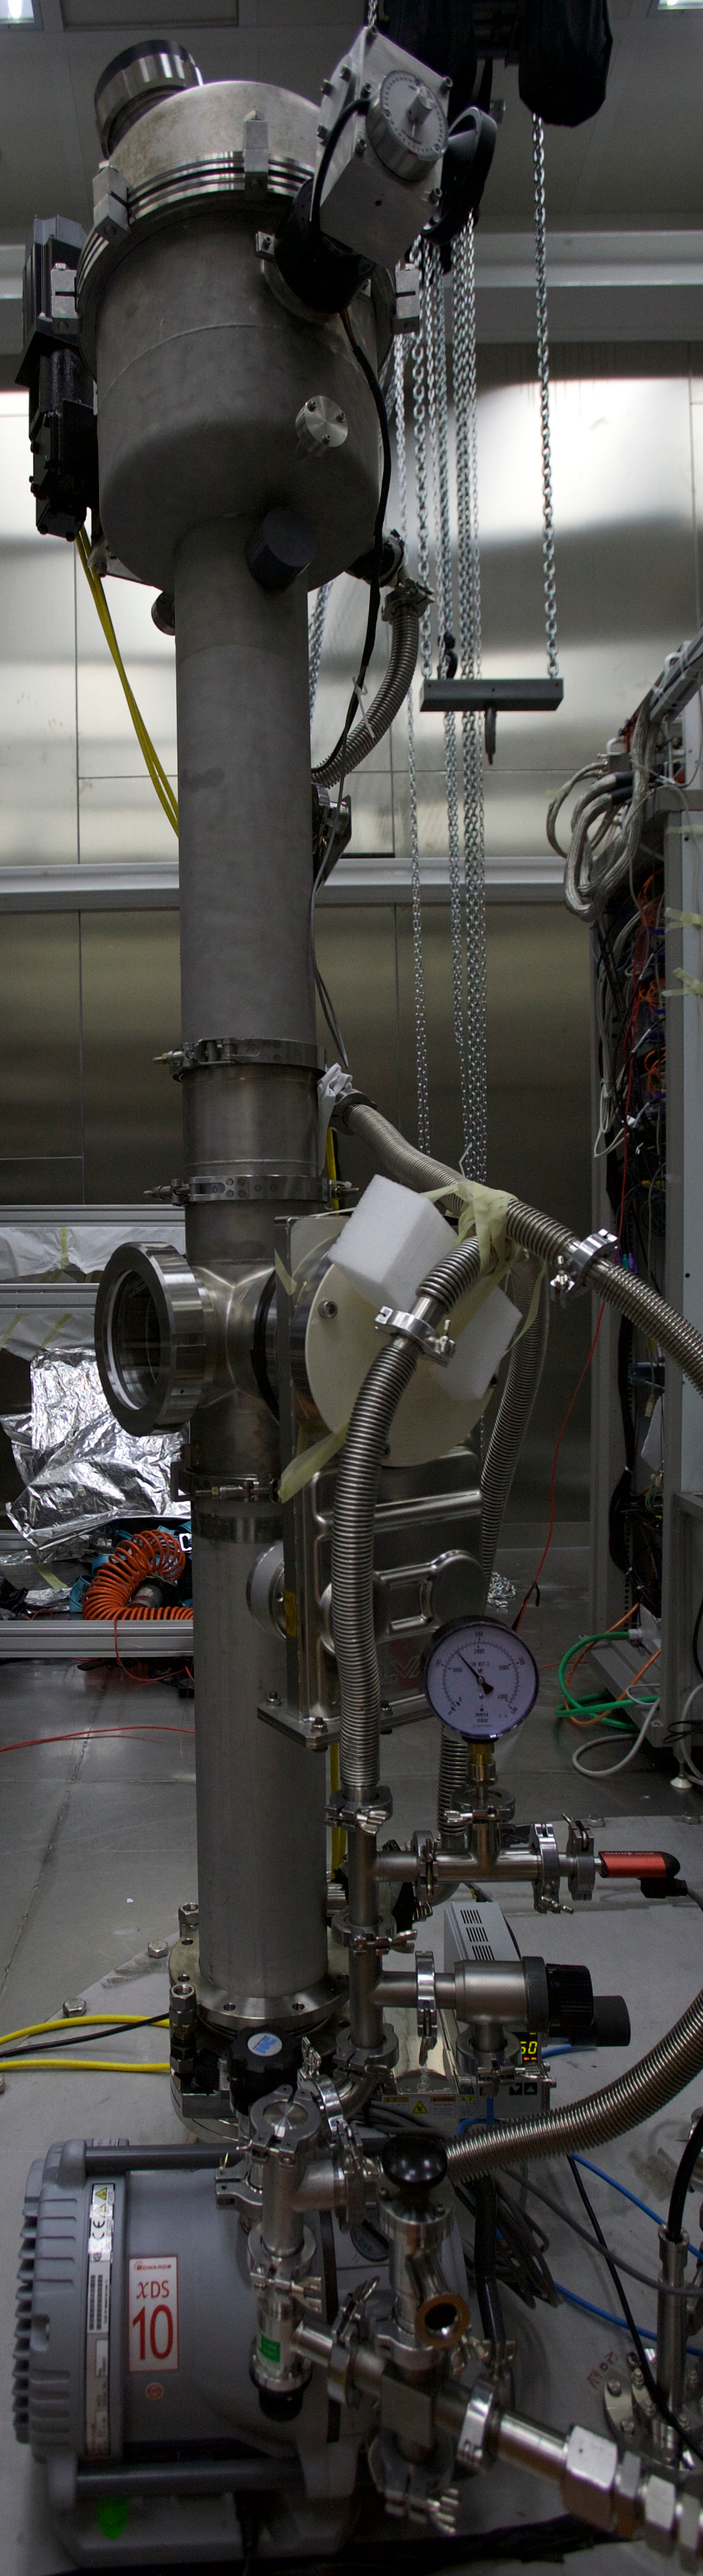
\includegraphics[width=0.25\textwidth]{Figures/CALIS_overview_IMG_3763.JPG}
% \caption{Flushing and nitrogen purging system.}
% \label{fig:flushing_purging}
%\end{figure}

\subsubsection*{Material Compatibility}
All materials coming in contact with the scintillator veto are made of stainless steel or teflon except for the sealing o-rings which are made of viton.  All three materials are certified materials for contact with all scintillator components including TMB and PC.

\subsection{Deployment Device}
The deployment device (Fig. \ref{fig:CALISMechanism}) contains the mechanical support structure for the source arm, which holds the calibration source at its end. The device is equipped with tapered cones on its top and bottom ensuring that ends do not get snagged on inner edges as it moves down and up, such as when reentering the organ pipe from the inside of the \lsv while on its way back to its home position. It is attached to the housing by two cables. Swivel hooks are employed in the attachment of the cables to the deployment device allowing them to move freely and not get tangled. 
There are two weights built into the device, one cylindrical in the conical cap above the rotation gear mechanism and one inside the cones at the device's bottom end. Both help to minimize any lateral motion or oscillations during deployment, articulation and dearticulation especially. It also ensures smooth motion of the deployment device into the organ pipe and back to the home position inside the CALIS housing.

\subsection{Source Holder and Arms}
A source arm and source holder are attached to an articulation gear (Fig.~\ref{fig:SourceHolder}). Different arm lengths have been prepared with a maximum arm length of 62 cm, arm length thereby being measured from the pivot point of the rotation gear to the source holder's tip. This arm length allows the source to be placed in immediate contact with the cryostat (Fig.~\ref{fig:CALIS_photos}, right), since the organ pipe's center axis is 80 cm from the TPC center and the cryostat has an outer radius of 32 cm. The 62 cm arm was used for deployments in past calibration campaigns (Sec.~\ref{sec:CalibCampaigns}). Inside the source holder the radioactive source is placed. During deployment, articulation and dearticulation it is pressed to the tip and held in place via a spring. The source holder is sealed such that no liquid scintillator can enter during deployment. This has also been verified during each source extraction and no liquid traces have been found in the holder's inside.

\begin{figure}[htbp]
 \centering
  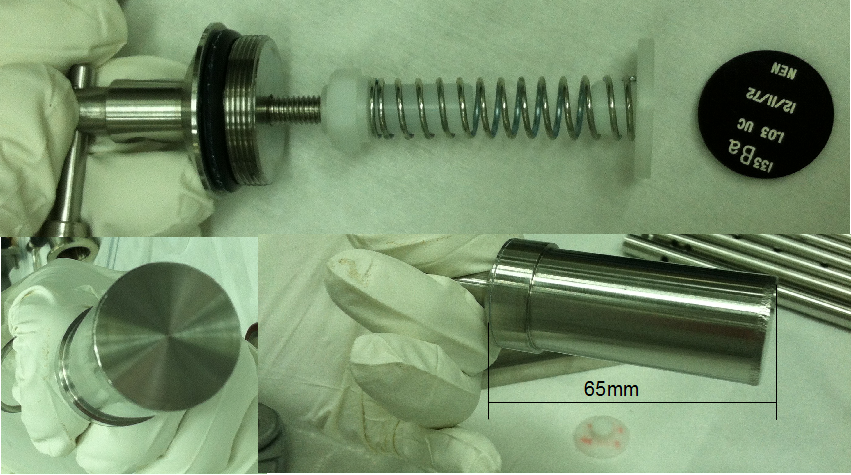
\includegraphics[width=0.7\textwidth]{Figures/SourceHolder.png}
  \caption{The source holder that connects to an arm and to the articulation gear of the deployment device. The source, here a $^{133}$Ba source, is pressed to the tip of the source holder via a spring.}
  \label{fig:SourceHolder}
\end{figure}